%----------createPrimitiveType----------------------------------------
\op
{createPrimitiveType}
{creates a new primitiveType}
{createPrimitiveType(Package selectedEObject, String nameValue, String idValue)}
{The package providing the container for the newly created primitiveType.}
{
\begin{itemize}
 \item nameValue/newName: The name of the newly created primitiveType
 \item idValue/newID: The id of the newly created pimitiveType
\end{itemize}
}
{There is no primitiveType whose name equals the parameter-value of 'newName' (see
\ref{subsec:checkOtherNames})}
{The name and the id will be set via input data.}
\begin{figure}[H]
  \centering
  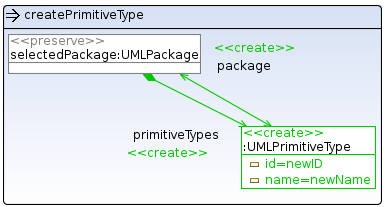
\includegraphics[width=0.65\textwidth]{pics/createPrimitiveType.png}
  \caption{createPrimitiveType}
  \label{createPrimitiveType}
\end{figure}
%----------deletePrimitiveType----------------------------------------
\op
{deletePrimitiveType}
{Deletes a primitiveType}
{deletePrimitiveType(PrimitiveType selectedEObject)}
{The primitiveType which should be deleted}
{-}
{-}
{For a better readability this is a simplified version of the
'deletePrimitiveType'-transformation and will only cover cases where the
primitiveType has no references to other elements. Such a
complex transformation rule exits but won't be listed here.}
\begin{figure}[H]
  \centering
  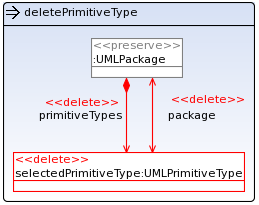
\includegraphics[width=0.4\textwidth]{pics/deletePrimitiveType_emptyAndUnreferenced.png}
  \caption{deletePrimitiveType}
  \label{deletePrimitiveType}
\end{figure}
%----------editPrimitiveTypeName----------------------------------------
\op
{editPrimitiveTypeName}
{edits the name of a primitiveType}
{editPrimitiveTypeName(PrimitiveType selectedEObject, String nameValue)}
{The primitiveType whose name should be renamed.}
{
\begin{itemize}
 \item nameValue/newName: The new name
\end{itemize}
}
{There is no primitiveType in the same package whose name equals the parameter-value of
'newName' (see \ref{subsec:checkOtherNames})}
{The \textless\textless create\textgreater\textgreater  -symbol in the image
means that even if the attribute exists its value will be overwritten.
'newName' is the placeholder for the input name.}
\begin{figure}[H]
  \centering
  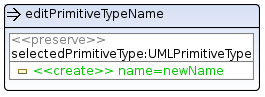
\includegraphics[width=0.4\textwidth]{pics/editPrimitiveTypeName.png}
  \caption{editPrimitiveTypeName}
  \label{editPrimitiveTypeName}
\end{figure}
%----------movePrimitiveType----------------------------------------
\op
{movePrimitiveType}
{moves a primitiveType from a package to another package}
{movePrimitiveType(PrimitiveType selectedEObject, Package tgt)}
{The primitiveType which should be moved.}
{
\begin{itemize}
 \item tgt/tgt[movePrimitiveType]: the target package
\end{itemize}
}
{There is no primitiveType with the same name in the target context (see
\ref{subsec:checkOtherNames})}
{Only references will change}
\begin{figure}[H]
  \centering
  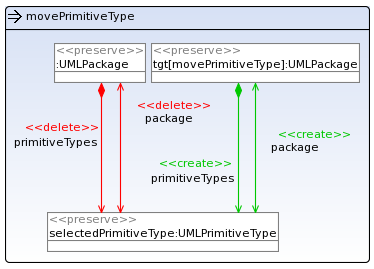
\includegraphics[width=0.65\textwidth]{pics/movePrimitiveType.png}
  \caption{movePrimitiveType}
  \label{movePrimitiveType}
\end{figure}